% \documentclass{standalone}
% \usepackage[dvipsnames]{xcolor}
% \usepackage{tikz}
% \usetikzlibrary{arrows.meta}

% \begin{document}

\tikzstyle{mybox} = [inner sep=1pt]

% Top row: A and B
\begin{subfigure}[t]{0.47\textwidth}
    % Panel A
    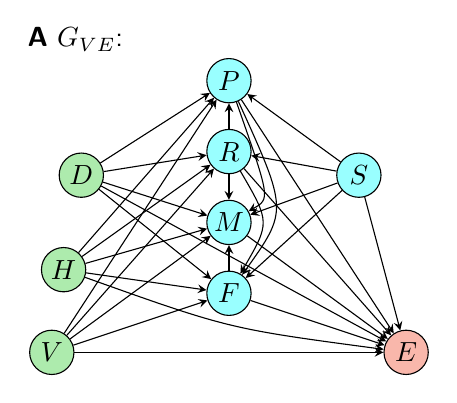
\begin{tikzpicture}[scale=0.75, inner sep=0pt]
      \node[inner sep = 0, font=\sffamily] (panel A) at (-2.6,5.3) {\textbf{A} $\mathbb{G}_{VE}$:};
      \node[circle, draw, fill=LimeGreen, text opacity=1, fill opacity=0.4, minimum width=16pt] (V) at (-3,0) {\(V\)};
      \node[circle, draw, fill=RedOrange, text opacity=1, fill opacity=0.4, minimum width=16pt] (E) at (3,0) {\(E\)};
      \node[circle, draw, fill=LimeGreen, text opacity=1, fill opacity=0.4, minimum width=16pt] (H) at (-2.8,1.4) {\(H\)};
      \node[circle, draw, fill=LimeGreen, text opacity=1, fill opacity=0.4, minimum width=16pt] (D) at (-2.5,3) {\(D\)};
      \node[circle, draw, fill=Cyan, text opacity=1, fill opacity=0.4, minimum width=16pt] (F) at (0,1) {\(F\)};
      \node[circle, draw, fill=Cyan, text opacity=1, fill opacity=0.4, minimum width=16pt] (M) at (0,2.2) {\(M\)};
      \node[circle, draw, fill=Cyan, text opacity=1, fill opacity=0.4, minimum width=16pt] (R) at (0,3.4) {\(R\)};
      \node[circle, draw, fill=Cyan, text opacity=1, fill opacity=0.4, minimum width=16pt] (P) at (0,4.6) {\(P\)};
      \node[circle, draw, fill=Cyan, text opacity=1, fill opacity=0.4, minimum width=16pt] (S) at (2.2,3) {\(S\)};

      % Edges from D
      \draw [-stealth] (D) edge (E);
      \draw [-stealth] (D) edge (F);
      \draw [-stealth] (D) edge (M);
      \draw [-stealth] (D) edge (P);
      \draw [-stealth] (D) edge (R);

      % Edges from F
      \draw [-stealth] (F) edge (E);
      \draw [-stealth] (F) edge (M);

      % Edges from M
      \draw [-stealth] (M) edge (E);

      % Edges from P
      \draw [-stealth] (P) edge (E);
      \draw [-stealth] (P) .. controls (1, 2.4) .. (F);
      \draw [-stealth] (P) .. controls (0.7, 2.6) .. (M);

      % Edges from R
      \draw [-stealth] (R) edge (E);
      \draw [-stealth] (R) .. controls (0.7, 2.2) .. (F);
      \draw [-stealth] (R) edge (M);
      \draw [-stealth] (R) edge (P);

      % Edges from S
      \draw [-stealth] (S) edge (E);
      \draw [-stealth] (S) edge (F);
      \draw [-stealth] (S) edge (M);
      \draw [-stealth] (S) edge (P);
      \draw [-stealth] (S) edge (R);

      % Edges from V
      \draw [-stealth] (V) edge (E);
      \draw [-stealth] (V) edge (F);
      \draw [-stealth] (V) edge (M);
      \draw [-stealth] (V) edge (R);
      \draw [-stealth] (V) edge (P);

      % Edges from H
      \draw [-stealth] (H) .. controls (0, 0.4) .. (E);
      \draw [-stealth] (H) edge (F);
      \draw [-stealth] (H) edge (M);
      \draw [-stealth] (H) edge (P);
      \draw [-stealth] (H) edge (R);
    \end{tikzpicture}
\end{subfigure}
\hspace{-5em}
\begin{subfigure}[t]{0.47\textwidth}
    % Panel B
    \begin{tikzpicture}
      \node[inner sep = 0, font=\sffamily] (panel B) at (4.3,2.2) {\textbf{B} $\mathbb{C}_{VE}$:};
      \node [mybox, right =of E] (box){%
        \begin{minipage}[!t]{\textwidth}
          \footnotesize
          \openup -0.5ex
          \begin{equation} \label{eq:SCM_fig}
            \begin{aligned}
          V &\coloneq \mathcal{U}_V \\
          H &\coloneq \mathcal{U}_H \\
          D &\coloneq \mathcal{U}_D \\
          S &\coloneq \mathcal{U}_S \\
          R &\coloneq f_R(V, H, D, S, \mathcal{U}_R) \\
          P &\coloneq f_P(V, H, D, S, R, \mathcal{U}_P) \\
          F &\coloneq f_F(V, H, D, S, P, R, \mathcal{U}_F) \\
          M &\coloneq f_M(V, H, D, S, P, R, F, \mathcal{U}_M) \\
          E &\coloneq f_E(V, H, D, S, P, R, M, F, \mathcal{U}_E) \\
          \end{aligned}
          \end{equation}
        \end{minipage}
      };
    \end{tikzpicture}
\end{subfigure}

% Add vertical space between rows
\vspace{1em}

% Bottom row: C and D
\begin{subfigure}[t]{0.47\textwidth}
    % Panel C
    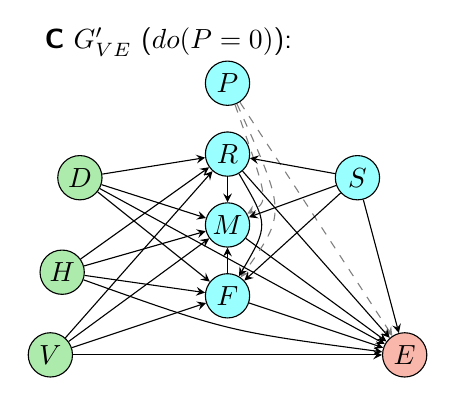
\begin{tikzpicture}[scale=0.75, inner sep=0pt, xshift=-1cm]
      \node[inner sep = 0, font=\sffamily] (panel C) at (-1,5.3) {\textbf{C} $\mathbb{G}'_{VE}$ ($do(P=0)$):};
      \node[circle, draw, fill=LimeGreen, text opacity=1, fill opacity=0.4, minimum width=16pt] (V) at (-3,0) {\(V\)};
      \node[circle, draw, fill=RedOrange, text opacity=1, fill opacity=0.4, minimum width=16pt] (E) at (3,0) {\(E\)};
      \node[circle, draw, fill=LimeGreen, text opacity=1, fill opacity=0.4, minimum width=16pt] (H) at (-2.8,1.4) {\(H\)};
      \node[circle, draw, fill=LimeGreen, text opacity=1, fill opacity=0.4, minimum width=16pt] (D) at (-2.5,3) {\(D\)};
      \node[circle, draw, fill=Cyan, text opacity=1, fill opacity=0.4, minimum width=16pt] (F) at (0,1) {\(F\)};
      \node[circle, draw, fill=Cyan, text opacity=1, fill opacity=0.4, minimum width=16pt] (M) at (0,2.2) {\(M\)};
      \node[circle, draw, fill=Cyan, text opacity=1, fill opacity=0.4, minimum width=16pt] (R) at (0,3.4) {\(R\)};
      \node[circle, draw, fill=Cyan, text opacity=1, fill opacity=0.4, minimum width=16pt] (P) at (0,4.6) {\(P\)};
      \node[circle, draw, fill=Cyan, text opacity=1, fill opacity=0.4, minimum width=16pt] (S) at (2.2,3) {\(S\)};

      % Edges from D
      \draw [-stealth] (D) edge (E);
      \draw [-stealth] (D) edge (F);
      \draw [-stealth] (D) edge (M);
      % \draw [-stealth, dashed, gray] (D) edge (P);
      \draw [-stealth] (D) edge (R);

      % Edges from F
      \draw [-stealth] (F) edge (E);
      \draw [-stealth] (F) edge (M);

      % Edges from M
      \draw [-stealth] (M) edge (E);

      % Edges from P
      \draw [-stealth, dashed, gray] (P) edge (E);
      \draw [-stealth, dashed, gray] (P) .. controls (1, 2.4) .. (F);
      \draw [-stealth, dashed, gray] (P) .. controls (0.7, 2.6) .. (M);

      % Edges from R
      \draw [-stealth] (R) edge (E);
      \draw [-stealth] (R) .. controls (0.7, 2.2) .. (F);
      \draw [-stealth] (R) edge (M);
      % \draw [-stealth, dashed, gray] (R) edge (P);

      % Edges from S
      \draw [-stealth] (S) edge (E);
      \draw [-stealth] (S) edge (F);
      \draw [-stealth] (S) edge (M);
      % \draw [-stealth, dashed, gray] (S) edge (P);
      \draw [-stealth] (S) edge (R);

      % Edges from V
      \draw [-stealth] (V) edge (E);
      \draw [-stealth] (V) edge (F);
      \draw [-stealth] (V) edge (M);
      \draw [-stealth] (V) edge (R);
      % \draw [-stealth, dashed, gray] (V) edge (P);

      % Edges from H
      \draw [-stealth] (H) .. controls (0, 0.4) .. (E);
      \draw [-stealth] (H) edge (F);
      \draw [-stealth] (H) edge (M);
      % \draw [-stealth, dashed, gray] (H) edge (P);
      \draw [-stealth] (H) edge (R);
    \end{tikzpicture}
\end{subfigure}%
\hspace{-5em}
\begin{subfigure}[t]{0.49\textwidth}
    % Panel D
    \begin{tikzpicture}
      \node[inner sep = 5, font=\sffamily] (panel D) at (4.3,2.3) {\textbf{D} $\mathbb{C}'_{VE}$ ($do(P=0)$):};
      \node [mybox, right =of E] (box){%
        \begin{minipage}[!t]{\textwidth}
          \footnotesize
          \openup -0.5ex
          \begin{equation} \label{eq:SCMcounterfactual_fig}
            \begin{aligned}
          P & = 0 \\
          V & \coloneq \mathcal{U}_V \\
          H & \coloneq \mathcal{U}_H \\
          D & \coloneq \mathcal{U}_D \\
          S & \coloneq \mathcal{U}_S \\
          R & \coloneq f_R(V, H, D, S, \mathcal{U}_R) \\
          F & \coloneq f_F^{P=0}(V, H, D, S, R, \mathcal{U}_F) \\
          M & \coloneq f_M^{P=0}(V, H, D, S, R, F, \mathcal{U}_M) \\
          E & \coloneq f_E^{P=0}(V, H, D, S, R, M, F, \mathcal{U}_E) \\
          \end{aligned}
          \end{equation}
        \end{minipage}
      };
    \end{tikzpicture}
\end{subfigure}

% \end{document}
